
\section{Overview}
%We're finding planets at an ever increasing rate.
When my parents gave me my first books on astronomy, the glossy pages were filled with fantastic color images from the Viking, Galileo, and Voyager missions, cataloging all of the known worlds beyond Earth. Everything there was to know about planets was wrapped up neatly into books about those (then nine) planets. At the same time -- eleven months before I began kindergarten -- the first planet orbiting Sun-like was discovered, 51 Pegasi b \citep{Mayor1995}. This new world, called an exoplanet -- or a planet that orbit a star other than the Sun -- would be the first of many. In the following years, the number of known planets would rise at an exponential rate through to the present. I am a member of the first generation for whom there has never been a time in our lives when our age in years has exceeded the number of known planets.

%We can characterize exoplanets with following techniques.
Exoplanets have been discovered principally via the transit method. This technique requires precise measurements of stellar brightness, or photometry, to discover worlds. The arcs of some exoplanet orbits bring the worlds between their host stars and the Earth -- allowing us to see an eclipse of the host star by the exoplanet, an event known as a transit. Precision photometry can reveal the small decrease in apparent brightness of the host star during the eclipse. 

Transit events transmit valuable information about exoplanets. The fraction of light missing during a transit event is simply the ratio of cross-sectional areas of the planet and star, $\Delta F/F \approx (R_p/R_\star)^2$, revealing the ratio of the planetary and stellar radii. For example, an Earth-sized planet orbiting a Sun-sized star only obscures 0.008\% of the brightness of the star. The time between transit events is the orbital period of the planet, which is related to the distance between the planet and its host star, or the orbital semi-major axis, via Kepler's third law. With the orbital separation and a bit of knowledge about the host star's luminosity, we can make a crude estimate of the equilibrium temperature of the planet -- and thus whether or not it might be a world suitable for life.

%But we only know as much about planets as we know about their host stars. 
In short order, we have already discovered that we can only know as much about a planet as we know about its host star. The planet's radius is measured relative to the stellar radius, and the planet's temperature is estimated relative to the stellar luminosity (and other terms). In order to make robust statements about exoplanets and their habitability, we must know a few things about their stars first.  

%Here's how we generally know about exoplanet host stars. 
Customarily, exoplanet hosting stars are given cursory characterization upon discovery of their planets. This basic reconnaissance might include the use of broad-band photometry (color) to estimate the temperature of the star, and parallactic distances to measure the stellar luminosity when available, in combination with expensive high resolution spectroscopy to identify the evolutionary state of the star. These measurements give an estimate of the stellar mass and radius, allowing us to estimate the absolute radius of the planet -- which is often used to confirm its nature as a planetary body, rather than a larger object like a brown dwarf or small star -- and its surface temperature. 

For a subset of these planets, we can also learn their masses using radial velocity measurements of the host star. If the planet is massive enough or close enough to its host star, and the host star isn't particularly active (more on this later), the gravitational acceleration of the star due to the planet is detectable via spectroscopy by looking for small Doppler shifts in the stellar spectrum. The acceleration of the star is related to the distance and mass of the exoplanet. If the planet is a transiting exoplanet, we know the orbital distance already via Kepler's third law, by knowing the planet's orbital period and the host star's mass, and thus we get a direct measurement of the mass of the planet. Combining the mass and radius measurements, we can get bulk density measurements of an exoplanet, indicating perhaps whether it is rocky or gaseous \citep{Seager2007}. 

% We can measure masses with TTVs
In transiting multi-planet systems, we can measure the masses of exoplanets without expensive spectroscopy by using transit timing variations (TTVs) \citep{Agol2005,Holman2005}. The orbit of a single transiting planet around a single star would be perfectly periodic (barring relativistic effects), but if there is more than one planet in the system, the gravitational influence of each planet on each other pulls the planets slightly ahead or behind in their orbits. The apparent early or late arrival of an exoplanet transit thus transmits information about the mass of the perturbing planet. This technique is especially promising for measuring the masses of small planets in the habitable zones of their Sun-like host stars -- which are typically too far and have too little mass to impart measurable radial velocities on their host stars with current high resolution spectroscopy. 

% We can measure atmospheric composition with transmission spectroscopy
Transits can also reveal the composition of exoplanet atmospheres via transmission spectroscopy \citep{Seager2000}. When the planet passes in front of the host star, the planet will appear largest at wavelengths where the planet's atmosphere is opaque, and smallest at wavelengths where the atmosphere is transparent. Thus by measuring the apparent radius of the planet as a function of wavelength, we can obtain a spectrum of an exoplanet's atmosphere. Encoded in this spectrum are absorption features from the atoms and molecules in the planet's upper atmosphere, yielding clues to the atmospheric composition, and the state of the planet's climate. 

% Astrobiology
The search for life in the Universe is the ultimate motivation for the work presented in this dissertation. We fix our  attention on the second major question of the NASA Astrobiology Roadmap: does life exist elsewhere in the Universe \citep{DesMarais2008}? The search for life may be guided by observations of transiting exoplanets, for example: by using TTVs to discover the bulk compositions of habitable exoplanets and determine which planets have surfaces; or by using transmission spectroscopy to search for biosignatures, or signs of life, in exoplanet atmospheres. These critical first measurements may indicate whether a planet simply resides in its host star's habitable zone or is in fact potentially habitable. 

%Stars are active. Here's what stellar activity is.
Thus far, our triumphant narrative of planet characterization has glided over some increasingly important details about the stars, which we have taken for granted as simple, uniform disks. One planet-hosting star has been studied for thousands of years: the Sun. Even before the invention of the telescope it was known that the Sun bares dark spots on its surface \citep{Hayakawa2017}. Sunspots are regions in the solar photosphere where strong magnetic fields inhibit convection of hot plasma from below, inhibiting heat transport and creating cool, dark spots on the Sun's surface \citep{Solanki2003}. As the Sun rotates, sunspots roll into and out of view, subtly changing the light we receive from the Sun as a function of wavelength and time.

% Planet-hosting are active.
Since the time of Copernicus, astronomical advances consistently remind us that the Earth is not at the center of the Universe, and that there is nothing particularly special about our location \citep{Copernicus1543} -- so perhaps it is no surprise that the Sun and Solar System are not unique. Multi-planet systems like ours are common \citep{Dressing2013,Burke2015,Coughlin2016}. The processes that drive magnetic activity on the Sun, or analogous ones for smaller stars, are also ubiquitous among planet-hosting stars. The evidence for those starspots comes to us from photometry -- the same technique used to discover planets -- revealing the changes in brightness as spotted planet-hosting stars rotate, for example, with photometry from NASA's \kepler mission \citep{Walkowicz2013,McQuillan2013,Giles2017}.  

% We can study stellar magnetic activity like this.
Detecting the sizes and temperatures of starspots is difficult. For main sequence stars, the angular resolution required for a telescope to spatially resolve starspots is beyond the diffraction limit for even the largest telescopes in the optical and infrared. Clever analysis of stellar spectral absorption features can reveal the positions of spots through Doppler imaging \citep{Vogt1983,Barnes2001,Strassmeier2002}, or its magnetic equivalent Zeeman Doppler imaging \citep{Donati2003,Morin2008,Morin2010,Morin2011,Morin2013}. Alternatively, one can measure the spot temperatures and covering fractions from high resolution spectra of active stars with molecular band modeling. The observed spectrum of a star is modeled as a linear combination of model or template stellar atmospheres with a hot and cooler component \citep{Neff1995,oneal1996,oneal1998,ONeal2004}. 

Another window into stellar magnetic activity was opened by \kepler transit photometry. During a transit event, when a planet occults a dark starspot, less light is missing than during occultations of brighter regions, creating a positive residual signal in transit light curves. One planet has revealed more about its star's spots than any other known to date, HAT-P-11 b \citep{Bakos2010,Winn2010,Deming2011,Sanchis-Ojeda2011,Hirano2011}. 

% Stellar activity affects exoplanet characterization in the following ways
Starspots directly affect our ability to make precise measurements of exoplanet properties. Their effect on the stellar flux adds signal of similar amplitude to the transit of an Earth-like planet for some Sun-like stars, making precise measurements of the transit depths (with photometry or transmission spectroscopy) and transit times (for TTVs) more challenging. To make matters worse, spots are cooler than the mean photosphere, introducing a wavelength-dependence to the variability in addition to time-dependence. Careful analyses of exoplanet properties must account for the effects of starspots in order to make reliable inferences about exoplanets. 

\section{Astrobiology} \label{sec:ab}

% Define astrobiology
Astrobiology is the study of the origin and evolution of life on the Earth, and the search for conditions amenable to life elsewhere in the Universe. Life thrives in a bewildering variety of environments on Earth, from the bitter cold of Earth's ice caps to the boiling heat of submarine hydrothermal vents \citep{Rothschild2001,Cavicchioli2002}. It seems that one of the few criteria that life on Earth universally demands is the presence of some liquid water \citep{DesMarais2002}. 

% define HZ
As a result, the search for life in the Universe thus far has focused on planets that reside in their host star's ``habitable zone'' -- or the range of orbital distances on which a planet may sustain liquid surface water \citep[e.g.][]{Huang1959,Kasting1993,Kopparapu2013}. The inner edge of the habitable zone is often defined as the orbital distance where a terrestrial planet's atmosphere warmed by a runaway greenhouse-effect would create surface conditions too hot to sustain liquid water. The outer edge is often defined by the orbital distance where a dense atmosphere of greenhouse gases provides insufficient warming to maintain liquid water at the planet's surface.
For the purposes of this dissertation, planets which fall between these two orbital distances defined by climatic catastrophes will be referred to as ``potentially habitable.'' 

% define problems of studying habitable worlds 
Perhaps the first detections of life on another planet will come from searches for planets with global-scale biospheres which affect the entire atmosphere or surface of a planet, just as life shapes the present-day mixing ratios of the Earth's atmospheric constituents, and Earth's albedo \citep{Sagan1993}. Such a biosphere could be detected with modern technology via transmission spectroscopy or direct imaging of an exoplanet, for example. Both of these techniques rely upon transmitted or reflected light from the host star interacting with the atmosphere of the planet to spectroscopically reveal biosignatures, or signs of life. We will show in the following sections that signals generated by magnetic activity and variability of the host star may confound our best attempts to characterize exoplanet atmospheres. 

TRAPPIST-1 is an exemplary system for demonstrating how uncertainties surrounding a stellar atmosphere propagate into uncertainties regarding planetary atmospheres. TRAPPIST-1 is the M8V host star to at least seven transiting, Earth-sized planets in a resonant chain, some of which reside in the habitable zone \citep{Gillon2016,Gillon2017,Luger2017}. Spectrophotometry during transits has revealed little about the atmospheres of the TRAPPIST-1 planets \citep{deWit2016, Ducrot2018}, due in part to significant contamination of the transmission spectra by the apparent presence of active regions on the stellar surface \citep{Morris2018c, Zhang2018, Wakeford2019}. 

One of the goals of this dissertation is to understand the effects of stellar magnetic activity and variability on observations of exoplanets, so that exoplanets may be characterized accurately in the presence of host stars with heterogeneous surfaces. A distant observer looking at the Solar System would be best prepared to accurately recognize the Earth as a potentially habitable exoplanet, for example, if they knew how to identify and remove the astrophysical signals generated by the Sun. 

The Sun is our local laboratory for understanding stellar oscillations, magnetic activity and the dynamo which powers that activity. In the next three sections we briefly introduce the mechanisms responsible for the Sun's long-term photometric variability from scales of months to years, by summarizing the history of sunspot observations in Section~\ref{intro:spots}, the magnetohydrodynamics of sunspots in Section~\ref{intro:mhd}, and a description of the dynamo mechanism which gives rise to sunspots' cyclic behavior in Section~\ref{sec:solardynamo}. In Section~\ref{sec:shorttermvar} we focus on the myriad short-term sources of solar variability from minutes to days, and we conclude the introduction with an outline of this dissertation in Section~\ref{sec:outline}.

\section{Sunspots} \label{intro:spots}

Sunspots have been observed on the Sun with the naked eye for millennia and with the telescope since Galileo. Since we can spatially resolve sunspots and study their substructure in detail, sunspots form the foundation of our understanding of starspots in general. In this Section we will briefly outline historical milestones in the study of sunspots.  

We recently marked the 400\textsuperscript{th} anniversary of Galileo's observation that the Sun has dark spots on its surface, which rotate into and out of view \citep{Galilei1613}. Astronomers continued to monitor the dark spots on the solar surface from the mid-seventeenth century onwards, typically by counting the number of starspots observed on the Sun. Thus the most enduring measurement in heliophysics is the ``sunspot number'' (SSN). 

Incredibly, the cyclic nature of the SSN was discovered by a pharmacist-turned-astronomer who was in fact searching for a transiting planet in the Solar System. From 1826 to 1843, Samuel Heinrich Schwabe sketched observations of the Sun on every clear day, searching for solar transits of a hypothesized planet interior to Mercury. While no planet appeared, Schwabe noted that the number of sunspots increases and decreases until no spots are visible, with an approximately period of 10 years \citep{Schwabe1844}. Spurred by Schwabe's discovery of the solar activity cycle, J. Rudolf Wolf compiled all of the available records of sunspots in order to measure the cycle period period, and found it to be 11 years long \citep{Wolf1852}.

Alexander Wilson recorded telescopic observations of starspots as they traverse the solar surface due to rotation. He noted that spots appear largest at disk-center, and smaller at the solar limb. He discovered that geometrical foreshortening due to the spherical surface of the Sun was insufficient to explain the small size of the spots at the limb. He posited that sunspots are troughs in the solar photosphere, and their depth obscures part of the spot from view at extreme viewing angles, discovering what we now call the Wilson depression \citep{Wilson1774}. 

The observation that spots are highly magnetized was first made by \citet{Hale1908}. Hale went to great lengths to study the Zeeman effect -- the apparent splitting of certain spectral lines in the presence of strong magnetic fields -- both in the laboratory and using spectroscopic observations of the Sun. He found that sunspots often occur in pairs of opposite magnetic polarity, which today is known as Hale's law \citep{Hale1925}.

\section{The Magnetohydrodynamics of Sunspots} \label{intro:mhd}

After Hale's discovery that starspots are magnetized he and colleagues, notably Sir John Larmor, asked the question ``how could a rotating body such as the Sun become a magnet?'' \citep{Larmor1919}. This question is a vexing one as it requires three-dimensional magnetohydrodynamics to solve. In the following section, we will briefly outline the mechanism by which starspots arise. 

The plasma in the outer convective zones of main sequence stars is conducting and magnetized, so its dynamics are dictated by Maxwell's equations: 
\begin{eqnarray}
\nabla \times \vec{E} &=& -\frac{\partial \vec{B}}{\partial t}\\
\nabla \times \vec{B} &=& \mu_0 \vec{J}\\
\vec{J}/\sigma &=& \vec{E} + \vec{v} \times \vec{B}\\
\frac{\partial \vec{B}}{\partial t} &=& \nabla \times \left( \vec{v} \times \vec{B} - \eta \nabla \times \vec{B} \right)
\end{eqnarray}
Where $\vec{E}$ and $\vec{B}$ are the electric and magnetic field vectors, $\vec{J}$ is the current vector, $\vec{v}$ is the plasma velocity, and $\eta$ is the magnetic diffusivity. The last relation, known as the induction equation, determines how the magnetic field evolves in time. On the right hand side, the first term, $\vec{v} \times \vec{B}$ is a source of inductance from bulk flow of the plasma, while the second term $\eta \nabla \times \vec{B}$ is a dissipative loss term due to resistance in the plasma. Using order of magnitude characteristic velocities (km/s convective motion), convective length scales (the solar radius) and resistivity, we find that the magnetic Reynolds number Rm is quite large:
\begin{eqnarray}
\textrm{Rm} = \frac{\textrm{induction}}{\textrm{dissipation}} = \frac{v L}{\eta}\\
v \sim 10^3\, \textrm{m s}^{-1}\\
L \sim R_\odot = 7 \times 10^8 \textrm{m}\\
\eta \sim 10^{0-5} \textrm{m$^2$ s}\\
\textrm{Rm} \sim 10^{6 - 10} \gg 1
\end{eqnarray}
\citep{Ossendrijver2003}. Thus in stars, the very high conductivity $\eta \rightarrow 0$ makes the dissipation term in the induction equation insignificant. In this regime we can apply the Alfv{\'e}n's ``frozen flux theorem'' \citep{Alfven1942}, which indicates that bulk flow of the plasma moves magnetic fields lines with it. This plays a critical role in the dynamics of plasma at the base of the convective zones in stars. The frozen flux theorem states that flux is conserved within an area $A$ before ($i$) and after ($f$) some stretching of the magnetic flux tube  
\begin{equation}
(B dA)_i = (B dA)_f,
\end{equation}
which can be combined with the conservation of mass for plasma of density $\rho$ in a flux tube of length $\ell$
\begin{equation}
(\rho \ell dA)_i = (\rho \ell dA)_f,
\end{equation}
to show that $B \propto \rho \ell$, or in words the magnetic field increases linearly with increasing length of the flux tube.

Now imagine a tube of plasma with magnetic field lines running along the length of it, at the base of the convective zone. Sun-like stars are differentially rotating -- the Sun, for instance, rotates once in 25 days at the equator, and closer to 34 days at the poles. Differential rotation of the star will stretch the plasma tube, making it longer and narrower, and since the frozen flux theorem applies, the plasma will drag the magnetic field lines with it, bringing the field lines closer together, i.e.\ amplifying the magnetic field in the flux tube. The pressure equilibrium between the plasma in the interior of the flux tube and the exterior medium is given by the plasma pressure in each region plus the magnetic pressure, $B^2/2\mu_0$, and using the ideal gas law, we can solve for the difference in density between the magnetic flux tube and its surroundings assuming $B_{\rm int} \gg B_{\rm ext}$:
\begin{eqnarray}
p_{\rm ext} + \frac{B_{\rm ext}^2}{2\mu_0} &=& p_{\rm int} + \frac{B_{\rm int}^2}{2\mu_0}\\
P &=& \rho \frac{kT}{m} \\
\rho_{\rm ext} - \rho_{\rm int} &=& \frac{B_{\rm int}^2}{2\mu_0} \frac{m}{kT}
\end{eqnarray}
We note that the term on the right hand side of the last equation is always positive for $B_{\rm int} > 0$, and thus the magnetized plasma will have a lower density than its surroundings, causing it to become buoyant and to rise. 

In this classical picture, a portion of the rising magnetic flux tube now rises through the convective zone, where it is subject to stochastic convective turbulence and the consistent twist of the Coriolis force, before it finally rises through the photosphere \citep{Rempel2011, Cheung2014}. The magnetic field is very strong at the two locations where the flux tube intersects the photosphere, giving rise to two regions where the local magnetic field dominates over convection. These are called bipolar magnetic regions (BMRs), as observations of the magnetic polarity of each region show opposite polarity, known as Hale's law -- a natural result of a single flux tube exiting (outward field) and entering (inward field) the photosphere. The halves of the BMRs are referred to as the leading and following components according to the direction of rotation. The twist of the Coriolis force causes BMRs to have a slight tilt with respect to a line of latitude, with the following component at higher latitudes than the leading component in the northern hemisphere (known as Joy's Law). Since the upwelling of hot plasma from convection is suppressed by the strong magnetic fields, an area just below the quiescent photosphere is evacuated, pushing the effective photosphere downwards, known as the Wilson depression. In regions of strong enough fields, the evacuated region cools and thus the cores of the BMRs are observed as dark sunspots. 

In summary, dark starspots are the magnetic footprints of strong magnetic fields, which originate at the base of the convective zone and rise through the photosphere due to magnetic buoyancy in differentially rotating stars. Spots often occur in pairs of opposite polarity known as bipolar magnetic regions which are slightly tilted with respect to lines of latitude.

\section{The Solar Dynamo} \label{sec:solardynamo}

In the previous section, we described the process by which a plasma tube with a magnetic field may rise through the surface and produce starspots observed in the photosphere. There is a problem lurking in our description of stellar magnetic fields -- stellar plasma is not in fact dissipationless, and in time, one might expect the bulk flows that give rise to amplified magnetic fields to decay due to resistance until fields are no longer produced. Or another challenge is the subject of how to construct a bulk flow of the plasma which remains magnetized, as it must not be axisymmetric in order to be sustained over millennia (known as Cowling's Theorem, see \citealt{Cowling1933}). In this section we'll briefly outline the mechanism known as the $\alpha  \Omega$ dynamo, which reproduces the observed solar magnetic activity cycle \citep{Hathaway2010, Charbonneau2014}. 

Suppose we start the Sun with a strictly dipolar field, like a bar magnet -- see Figure~\ref{fig:alpha_omega}. The real Sun does have a dipolar field at solar minimum. Field lines in the convective zone run along meridional lines in this initial condition -- or in other words the field is strictly poloidal. Since the Sun is differentially rotating, and the frozen flux theorem applies, the field lines near the equator are dragged ahead of the field lines near the poles. After several rotations, the originally meridional field lines have been twisted around the Sun several times, wound up like a spring at the mid-latitudes, until a significant component of the magnetic field is running along lines of latitude -- or in other words, there is a significant toroidal component of the magnetic field. The twisting of the meridional (poloidal) magnetic field lines into azimuthal (toroidal) ones due to differential rotation is known as the $\Omega$-effect. 

\begin{figure}
\centering
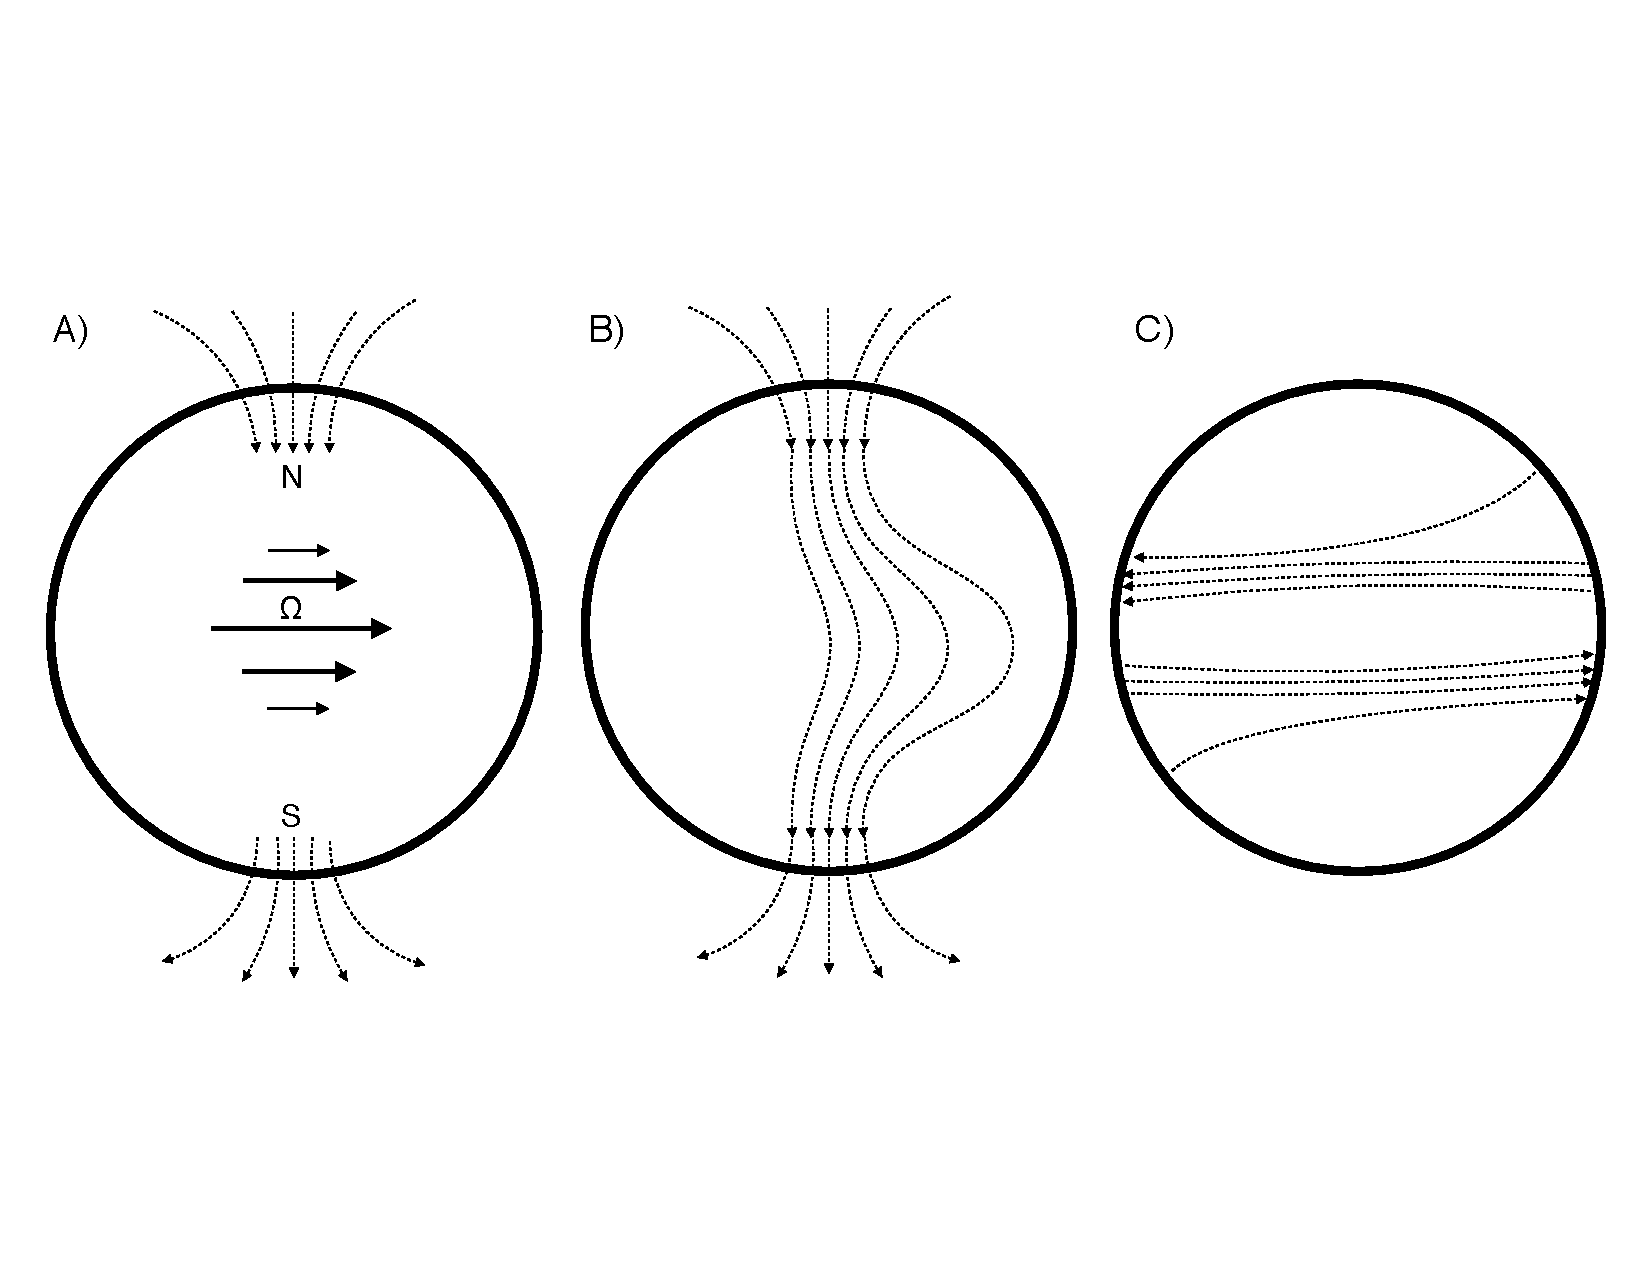
\includegraphics[scale=0.55]{intro/alpha_omega.pdf}
\caption{The conversion of poloidal to toroidal magnetic fields (dashed arrows) in a differentially rotating star (solid arrows). The star begins at A with a strictly poloidal field, like a bar-magnet. Since Alfv{\'e}n's ``frozen flux theorem''  applies, magnetic field lines are frozen into the plasma. The star is differentially rotating, meaning it rotates faster at the equator than at the poles, causing the magnetic field lines that were originally poloidal (A) to begin to twist after several rotations (B). After several more rotations (C), the magnetic field is tightly wound around the star several times and concentrated at the mid-latitudes. } \label{fig:alpha_omega}
\end{figure}

Now we have the magnetic field lines wrapped around the star and concentrated (amplified) at the mid-latitudes. As differential rotation continues to stretch the plasma and amplify the magnetic field, the flux tubes eventually become unstable and rise through the photosphere, producing starspots via the mechanism described in the previous section. Some of the magnetic flux tubes have a twist imparted on them by the Coriolis effect and by convective turbulence \citep{Parker1955a, Parker1955b}, which together create loops in the twisted magnetic flux tubes. Magnetic reconnection occurs, liberating the magnetic field loops, which due to the earlier twist now contain a poloidal component. This is known as the $\alpha$-effect. 

Now the simultaneously present toroidal and poloidal field components interact with each other, causing bands of magnetic flux tubes to migrate from the mid-latitudes towards the equator, creating the observed dynamo wave of starspots that first emerge at mid-latitudes (near 30$^\circ$) and drift towards the equator throughout the solar activity cycle \citep{Parker1955a, Parker1955b, Babcock1961}. 

It has been observed that meridional flow exists on the solar surface which flows from the equator to the poles at the surface, and via the continuity it is thought that meridional flow must also exist at the base of the convective zone from the poles to the equator. The inferred flow at the base of the convection zone is slow, about 1 m/s, which is roughly the speed needed for bulk flow of plasma to migrate from 30$^\circ$ latitude to the equator in 11 years -- causing some to speculate whether flux transport via the meridional flow is responsible for the 11 year periodicity of the solar activity cycle \citep{Dikpati2006,Hathaway2010}. 

\section{Short-Term Solar Variability} \label{sec:shorttermvar}

\begin{figure}
\centering
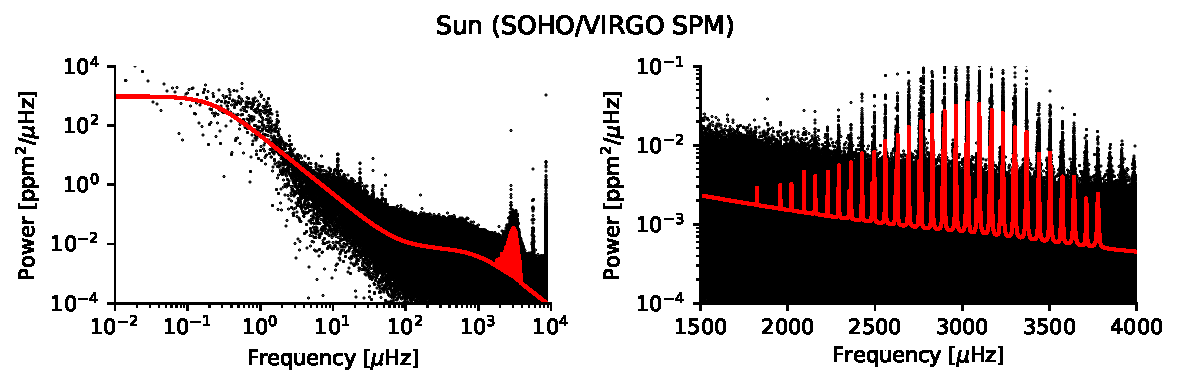
\includegraphics[scale=0.8]{intro/sun.pdf}
\caption{Solar variability as a function of frequency, measured by SOHO VIRGO/SPM \citep{Frohlich1997}. For the periodically inclined, we note: $10^{-2} \,\mu$Hz is equivalent to periods of 1150 days,  $1\,\mu$Hz is 11.5 days, $3000\,\mu$Hz is 5.5 minutes.} \label{fig:virgospm}
\end{figure}

The previous two sections summarize the emergence and dynamics of the Sun's magnetic active regions throughout the solar activity cycle, which drive photometric variability on timescales of months to years. The Sun is also variable on shorter timescales ranging from minutes to days. Figure~\ref{fig:virgospm} shows the power spectrum of solar broadband photometry taken over 20 years by the SOHO VIRGO/SPM instrument \citep{Frohlich1997}. There are three features in the solar power spectrum that we will encounter elsewhere in this dissertation (specifically in Chapters~\ref{chap:plato} and \ref{chap:astero}), which we summarize here \citep[see review by][]{Nordlund2009}. 

First we note the ``comb'' of peaks in the power spectrum in Figure~\ref{fig:virgospm} between 1000 and $4000\,\mu$Hz, with the greatest power near $3100\,\mu$Hz (period of 5.5 minutes). These peaks represent $p$-mode oscillations, or standing waves in the solar plasma for which the restoring force is pressure. The detection of these $p$-mode oscillations gave rise to the field of helioseismology, which makes use of the waves propagating throughout the solar atmosphere to measure fundamental properties of the Sun, including its internal structure \citep{Christensen-Dalsgaard2002}. Using simple scaling laws based on the solar $p$-mode oscillations, it is possible to predict properties of distant stars using short-cadence photometry \citep[e.g.][]{Kjeldsen1995,Kjeldsen2011,Huber2011,Huber2012,Kallinger2014}.

The next feature to note is the ``knee'' with near-constant power at mid-frequencies that begins to slope downward near $10^{3}\,\mu$Hz -- this is the signal of granulation. Granulation is the small-scale convective motion which gives rise to the numerous convective ``granules'' which tile the surface of the Sun. These granules are a few times the local scale height in horizontal extent, spanning a few Megameters (Mm). Granules produce power predominantly at periods $\lesssim30$ min.

The knee at the lowest frequencies near $10^{-1}\,\mu$Hz is due to supergranulation. Supergranulation is the signature of large-scale, slow convective motions which are generated by bulk flows roughly 20-40 Megameters (Mm) in size on the solar surface. Supergranules have the longest coherence timescale, giving rise to power in the power spectrum at periods $\lesssim10$ days. 

Each of these short-period solar photometric phenomena occur on other stars, and thus we can expect these signals to be present in short-cadence photometry of exoplanet host stars. In particular, we note that the ingress duration of an Earth orbiting a Sun-like star is roughly 10 minutes. Thus the periodic power generated by granulation and $p$-mode oscillations on timescales of order 10 minutes may affect the precision of observations of transiting Earth-like exoplanets, especially measurements such as transit timing variations which depend on precision at ingress and egress.

\section{Outline} \label{sec:outline}

In Part~\ref{part:solaractivity} we study the magnetic activity and variability of the Sun itself, and the impact of stellar variability and magnetic activity on observations of Earth-like exoplanets orbiting Sun-like stars. In Part~\ref{part:activity} we present detailed studies of the magnetic activity of distant stars, examining the effects of activity on transit photometry, high resolution spectroscopy and astrometry. %In Part~\ref{part:planets} we study a few transiting exoplanets using transit photometry to measure timing variations and starspot occultations. 
In Part~\ref{part:synthesis} we take advantage of our knowledge on stellar magnetic activity and exoplanet characterization to prepare for observations of planets orbiting active host stars. Finally we summarize our conclusions and outlook for future work in Part~\ref{part:conclusion}. 
